\documentclass[hyperref={hidelinks}]{beamer}

\setbeamertemplate{bibliography item}{\insertbiblabel}

\mode<presentation>

\usepackage{physics}
\usepackage{multimedia}
\usepackage{graphicx}
\usepackage{subcaption}
\usepackage{siunitx}
\usepackage{amsmath}
\usepackage{amssymb}
\usepackage[style=numeric-comp,backend=biber]{biblatex}
\usepackage{cleveref}
\usepackage{tikz}

\usetikzlibrary{patterns}

\addbibresource{biblio.bib}

\usefonttheme[onlymath]{serif}

%% For the Hindmarsh-Rose model
\newcommand*{\hrx}{x}
\newcommand*{\hry}{y}
\newcommand*{\hrz}{z}
\newcommand*{\hra}{\alpha}
\newcommand*{\hrb}{\beta}

%% For the chimera-like index
\newcommand*{\chimera}{\chi}
\newcommand*{\meta}{m}
\newcommand*{\ordparam}{r}
\newcommand*{\phase}{\phi}

\author{Henry Mitchell \inst{1,2,5} \and
  Peter Dodds \inst{1,4,5} \and
  Matt Mahoney \inst{3,4} \and
  Chris Danforth \inst{1,4,5}
}

\institute{
  \inst{1} Department of Mathematics and Statistics
  \inst{2} Department of Physics \\
  \inst{3} Department of Neurology
  \inst{4} Department of Computer Science \\
  \inst{5} Computational Story Lab
}

\titlegraphic{\includegraphics[width=2cm]{figure/roboctopus}\hspace*{4.75cm}~%
  \includegraphics[width=2cm]{figure/storylab}
}

\title{Chimera States and Seizures in a Mouse Neuronal Model}

\begin{document}

\frame{\titlepage}

\AtBeginSubsection[]{
  \begin{frame}
    \frametitle{Roadmap}
    \tableofcontents[currentsubsection]
  \end{frame}
}

\section{Introduction}

\subsection{Math}
\begin{frame}
  \frametitle{Synchronization}
  Huygens' pendulum clocks,
  fireflies,
  applauding crowds,
  people walking on London's Millenium Bridge,
  power grids,
  metronomes on a moving platform \ldots
  \begin{figure}[ht]
    \centering
    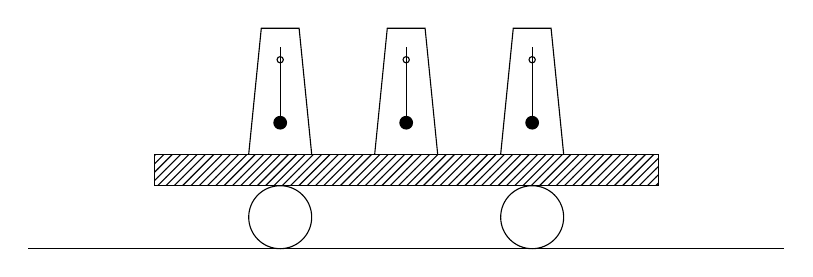
\begin{tikzpicture}[scale=0.8]
      \draw (0, 0) circle (0.5);
      \draw (4, 0) circle (0.5);
      \draw[pattern=north east lines] (-2, 0.5) -- (6, 0.5) -- (6, 1) -- (-2, 1) -- (-2, 0.5);
      \draw (-4, -0.5) -- (8, -0.5);
      \draw (-0.5, 1) -- ++(0.2, 2) -- ++(0.6, 0) -- ++(0.2, -2);
      \draw (0, 2.5) circle (0.05);
      \draw[fill] (0, 1.5) circle (0.1);
      \draw (0, 2.7) -- (0, 1.5);

      \draw (1.5, 1) -- ++(0.2, 2) -- ++(0.6, 0) -- ++(0.2, -2);
      \draw (2, 2.5) circle (0.05);
      \draw[fill] (2, 1.5) circle (0.1);
      \draw (2, 2.7) -- (2, 1.5);

      \draw (3.5, 1) -- ++(0.2, 2) -- ++(0.6, 0) -- ++(0.2, -2);
      \draw (4, 2.5) circle (0.05);
      \draw[fill] (4, 1.5) circle (0.1);
      \draw (4, 2.7) -- (4, 1.5);

    \end{tikzpicture}
    \label{fig:metronome_demo}
  \end{figure}
  All provide examples of synchrony in surprising places.

\end{frame}

\begin{frame}
  \frametitle{The Kuramoto Model}
  A commonly-used model where synchrony arises is the Kuramoto model:
  \begin{equation}
    \label{eq:kuramoto_phase}
    \pdv{t} \phi(x, t)
    =
    \omega
    -
    \int{G(x - x') \sin(\phi(x, t) - \phi(x', t) + \alpha) \dd{x'}}
  \end{equation}
  where
  \begin{equation}
    G(y)
    =
    \frac{\kappa}{2} e^{-k \abs{y}}
  \end{equation}
  It also exhibits some unexpected behavior\ldots

\end{frame}

\begin{frame}
  \frametitle{Chimera States}
  Chimera states are \textbf{the coexistence of synchronous and asynchronous populations within a network of nonlocally-coupled oscillators} \cite{Abrams2004,Kuramoto2002}.

  \begin{figure}[ht]
    \centering
    \begin{subfigure}{0.6\textwidth}
      \centering
      \includegraphics[width=\textwidth]{figure/kuramoto_overhead}
      \caption{The time series of the Kuramoto simulation.}
      \label{fig:kuramoto_overhead}
    \end{subfigure} %
    \begin{subfigure}{0.35\textwidth}
      \centering
      \includegraphics[width=\textwidth]{figure/kuramoto_snapshot}
      \caption{A snapshot at $t = 120$.}
      \label{fig:kuramoto_snapshot}
    \end{subfigure}
    \caption[Kuramoto simulation]{An example of a chimera state in a network of Kuramoto oscillators (coupling is proportional to sine of phase difference).
    }
    \label{fig:kuramoto_chimera}
  \end{figure}

\end{frame}

\begin{frame}
  \frametitle{Abrams Model}
  The Abrams Model is a network of Kuramoto oscillators divided into two populations.
  The coupling is stronger within populations than between them.
  \begin{equation}
    \label{eq:abrams}
    \dv{\theta_{i}^{\sigma}}{t}
    =
    \omega
    +
    \sum_{\sigma' = 1}^{2} \frac{K_{\sigma \sigma'}}{N_{\sigma'}} \sum_{j = 1}^{N_{\sigma'}} \sin(\theta_{j}^{\sigma'} - \theta_{i}^{\sigma} - \alpha)
  \end{equation}
  where
  \begin{equation}
    \label{eq:abrams_params}
    K
    =
    \bmqty{\mu & \nu \\ \nu & \mu}
    \qand
    \sigma \in \Bqty{1, 2}.
  \end{equation}

\end{frame}

\begin{frame}
  \frametitle{Abrams Simulation}
  \begin{figure}[ht]
    \centering
    \begin{subfigure}{0.6\textwidth}
      \centering
      \includegraphics[width=\textwidth]{figure/abrams_overhead}
      \caption{The time series of the Abrams simulation.}
      \label{fig:abrams_overhead}
    \end{subfigure} %
    \begin{subfigure}{0.3\textwidth}
      \centering
      \includegraphics[width=\textwidth]{figure/abrams_snapshot}
      \caption{A snapshot at $t = 799.45$.}
      \label{fig:abrams_snapshot}
    \end{subfigure}
    \caption[Abrams simulation]{A simulation of the Abrams model for two populations of 128 oscillators.
      (a) the time series of the simulation for $t \in \pqty{800, 1000}$.
      (b) a snapshot at $t = 799.45$.
    }
    \label{fig:abrams}
  \end{figure}

  This is with $\mu = 0.6$, $\nu = 0.4$, $\alpha = \frac{\pi}{2} - 0.05$.

\end{frame}

\begin{frame}
  \frametitle{A Mechanical Example}
  Two swinging platforms tied together with springs, each holding 15 metronomes.
  For certain strengths of the spring (coupling strengths), chimera states appeared \cite{Martens2013}.

  \vfill

  \movie[width=\textwidth,height=0.18\textwidth,autostart,loop=1]{A mechanical example of a chimera state}{figure/mechanical_chimera.mov}
\end{frame}

\begin{frame}
  \frametitle{Measures}
  A system's \textbf{order parameter} provides an instantaneous measure for how synchronous it is:
  \begin{equation}
    \label{eq:order}
    \ordparam(t)
    =
    \abs{\expval{e^{i \phase_{k}(t)}}_{k \in C}},
  \end{equation}
  where $\phase_{k}$ is the phase of oscillator $k$, and $\ev{f}_{k \in C}$ is the average of $f$ over all $k$ in community $C$.

\end{frame}

\begin{frame}
  \frametitle{Measures}
  There are two useful measures for determining how chimeric a system is:
  \begin{align}
    \label{eq:chimera}
    \chimera
    &=
      \expval{\sigma_{\text{chi}}}_{T}
    & \text{ where} \quad
      \sigma_{\text{chi}}(t)
    &=
      \frac{1}{M - 1} \sum_{c \in C}\pqty{\ordparam_{c}(t) - \expval{\ordparam_{c}}_{C}}^{2} \\
    \label{eq:metastability}
    \meta
    &=
      \expval{\sigma_{\text{met}}}_{C}
    & \text{ where} \quad
      \sigma_{\text{met}}(c)
    &=
      \frac{1}{T - 1} \sum_{t \leq T}\pqty{\ordparam_{c}(t) - \expval{\ordparam_{c}}_{T}}^{2}
  \end{align}
  The \textbf{chimera-like index} $\chimera$ is the time average of the variance between communities of the order parameter.
  Its maximum value is $1/7$, and will be normalized as such.

  The \textbf{metastability index} $\meta$ is the average across communities of the variance over time of the order parameter.
  Its maximum value is $1/12$, and will be normalized as such.

\end{frame}

\subsection{Brains}
\begin{frame}
  \frametitle{Neurons}
  Neurons are cells which are specialized for communication.
  They \textit{fire} by sending an electrochemical signal to other neurons.
  Internally, this \textit{action potential} is a set of fast excitatory processes and slow inhibitory processes.
  Neural firings are \textit{all-or-nothing}---a neuron can't half-fire.

  \vfill

  \begin{figure}[ht]
    \centering
    \includegraphics[width=\textwidth]{figure/action_potential}
    \caption{The membrane potential during a typical action potential.}
    \label{fig:action_potential}
  \end{figure}

\end{frame}

\begin{frame}
  \frametitle{Seizures}
  Seizures are \textbf{excessive(ly) synchronous neural activity} \cite{Kandel2013}.
  The two main types are:
  \begin{description}
  \item[Generalized] The entire brain enters ictal stage simultaneously

  \item[Focal] A subsection of the brain enters ictal stage while the rest remains asynchronous

  \end{description}

  Focal seizures often secondarily generalize.

\end{frame}

\subsection{Math and Brains}
\begin{frame}
  \frametitle{Brain Models}
  We have extremely accurate models for the behavior of individual neurons.
  But, more is different, and modeling brains as collections of individual neurons is impractical.
  So, we use mean-field approximations (and the like).

  This has two great benefits: %% Actually, it has way more than two benefits, but I'm highlighting two
  \begin{enumerate}
  \item Simpler to simulate

  \item Closer to observables

  \end{enumerate}

\end{frame}

\begin{frame}
  \frametitle{Epileptor}
  {\footnotesize
    A famous phenomenological seizure model is called Epileptor \cite{Jirsa2014}:
    \begin{align}
      \label{eq:epileptor_x1}
      \dot{x}_{1}
      &=
        y_{1}
        -
        f_{1}(x_{1}, x_{2})
        -
        z
        +
        I_{\text{rest} 1} \\
      \label{eq:epileptor_y1}
      \dot{y}_{1}
      &=
        y_{0}
        -
        5 x_{1}^{2}
        -
        y_{1} \\
      \label{eq:epileptor_z}
      \dot{z}
      &=
        \frac{1}{\tau_{0}} \pqty{4 \pqty{x_{1} - x_{0}} - z} \\
      \label{eq:epileptor_x2}
      \dot{x}_{2}
      &=
        -y_{2}
        +
        x_{2}
        -
        x_{2}^{3}
        +
        I_{\text{rest} 2}
        +
        0.002 g(x_{1})
        -
        0.3 \pqty{z - 3.5} \\
      \label{eq:epileptor_y2}
      \dot{y}_{2}
      &=
        \frac{1}{\tau_{2}} \pqty{-y_{2} + f_{2}(x_{1}, x_{2})}
    \end{align}
  }
  where
  {\tiny
    \begin{align}
      \label{eq:epileptor_g}
      g(x_{1})
      &=
        \int_{t_{0}}^{t}{e^{-\gamma \pqty{t - \tau}} x_{1}(\tau) \dd{\tau}} \\
      \label{eq:epileptor_f1}
      f_{1}(x_{1}, x_{2})
      &=
        \begin{cases}
          x_{1}^{3} - 3 x_{1}^{2},
          & \text{if } x_{1} < 0 \\
          x_{1} \pqty{x_{2} - 0.6 \pqty{z - 4}^{2}},
          & \text{if }
          x_{1} \geq 0
        \end{cases} \\
      \label{eq:epileptor_f2}
      f_{2}(x_{1}, x_{2})
      &=
        \begin{cases}
          0,
          & \text{if } x_{2} < -0.25 \\
          6 \pqty{x_{2} + 0.25},
          & \text{if } x_{2} \geq -0.25
        \end{cases}
    \end{align}
  }
  {\footnotesize
    and $x_{0} = -1.6$, $y_{0} = 1$, $\tau_{0} = 2857$, $\tau_{1} = 1$, $\tau_{2} = 10$, $I_{\text{rest} 1} = 3.1$, $I_{\text{rest} 2} = 0.45$, $\gamma = 0.01$.
  }

\end{frame}


\section{Methods}
\subsection{The Model}
\begin{frame}
  \frametitle{Model Parameters}
  \begin{table}[ht]
    \centering
    {\tiny
      \begin{tabular}{c | c | l}
        Symbol & Value & Meaning \\ \hline
        $\hrx_{j}$ & --- & \textbf{Membrane potential of the $j$th neural mass} \\
        $\hry_{j}$ & --- & \textbf{Associated with the fast processes} \\
        $\hrz_{j}$ & --- & \textbf{Associated with slow processes} \\ \hline
        $b$ & 3.2 & Tunes the spiking frequency \\
        $I_{j}$ & 4.4 & External input current \\
        $\hrx_{\text{rev}}$ & 2 & Ambient reverse potential \\
        $\lambda$ & 10 & Sigmoidal activation function parameter \\
        $\theta$ & -0.25 & Sigmoidal activation function parameter \\
        $\mu$ & 0.01 & Time scale for variation of $z$ \\
        $s$ & 4 & Governs adaptation \\
        $\hrx_{\text{rest}}$ & -1.6 & Resting/equilibrium potential \\ \hline
        $\hra$ & Varied & \textbf{Connection strength within cortices} \\
        $n_{j}'$ & \Cref{fig:connectome_matrix} & \textbf{Number of connections within a cortex from the $j$th neuron} \\
        $G_{j k}'$ & \Cref{fig:connectome_matrix} & \textbf{Intra-cortical connection matrix} \\
        $\hrb$ & Varied & \textbf{Connection strength between cortices} \\
        $n_{j}''$ & \Cref{fig:connectome_matrix} & \textbf{Number of connections between cortices from the $j$th neuron} \\
        $G_{j k}''$ & \Cref{fig:connectome_matrix} & \textbf{Inter-cortical connection matrix}
      \end{tabular}
      \caption[Hindmarsh-Rose Parameters]{The list of parameters used in modeling the Hindmarsh-Rose network.}
      \label{tab:hr_params}
    }
  \end{table}
\end{frame}

\begin{frame}
  \frametitle{The Model}
  We used a network of modified Hindmarsh-Rose neurons \cite{Santos2017}:
  \begin{align}
    \label{eq:hr_x}
    \begin{split}
      \dot{\hrx}_{j}
      ={}&
      \hry_{j}
      -
      \hrx_{j}^{3}
      +
      b \hrx_{j}^{2}
      +
      I_{j}
      -
      \hrz_{j} \\
      &\quad -
      \frac{\hra}{n'_{j}} \sum_{k ={} 1}^{N} G'_{j k} \Theta_{j}(\hrx_{k})
      -
      \frac{\hrb}{n''_{j}} \sum_{k ={} 1}^{N} G''_{j k} \Theta_{j}(\hrx_{k})
    \end{split} \\
    \label{eq:hr_y}
    \dot{\hry}_{j}
    ={}&
         1
         -
         5 \hrx_{j}^{2}
         -
         \hry_{j} \\
    \label{eq:hr_z}
    \dot{\hrz}_{j}
    ={}&
         \mu \pqty{s \bqty{\hrx_{j} - \hrx_{\text{rest}}} - \hrz_{j}}
  \end{align}
  where
  \begin{equation}
    \label{eq:hr_sigmoid}
    \Theta_{j}(\hrx_{k})
    =
    \frac{\hrx_{j} - \hrx_{\text{rev}}}{1 + e^{-\lambda \pqty{\hrx_{k} - \theta}}}
  \end{equation}
  This sigmoidal activation function helps make the model apply to groups of neurons (subcortices) instead of single neurons.

\end{frame}

\subsection{The Network}
\begin{frame}
  \frametitle{The Mouse Connectome}
  The oscillator network (\cref{fig:connectome}) was modeled after the mouse connectome \cite{Oh2014}.
  \begin{figure}
    \centering
    \begin{subfigure}{0.49\textwidth}
      \centering
      \includegraphics[width=0.99\textwidth]{figure/n}
      \caption{}
      \label{fig:connectome_matrix}
    \end{subfigure}%
    \begin{subfigure}{0.49\textwidth}
      \centering
      \includegraphics[width=0.99\textwidth]{figure/network}
      \caption{}
      \label{fig:connectome_embedding}
    \end{subfigure}
    \caption{(a) The mouse connectome represented as (a) a matrix and (b) a graph embedding.}
    \label{fig:connectome}
  \end{figure}

\end{frame}

\subsection{The Implementation}
\begin{frame}
  \frametitle{The Implementation}
  The Hindmarsh-Rose model was coded up in Python, and integrated for various values of $\hra$ and $\hrb$.
  The initial conditions were drawn from uniform distributions:
  \begin{equation*}
    \hrx_{j} \in \bqty{-2, 2}
    \qc
    y_{j} \in \bqty{0, 0.2}
    \qc
    z_{j} \in \bqty{0, 0.2}
  \end{equation*}
  Integrated over $\pqty{-1000, 5000}$, keeping $t \in \pqty{0, 4000}$.
  The first 1000 time units are to eliminate transients, and the last 1000 are calculated but discarded to facilitate calculation of the phase:
  \begin{equation}
    \label{eq:hr_phase}
    \phase_{j}(t)
    =
    2 \pi \times \frac{t - t_{i}}{t_{i + 1} - t_{i}}
  \end{equation}

\end{frame}

\section{Results}
\subsection{Model Quality}
\begin{frame}
  \frametitle{Real EEG output}
  \begin{figure}[ht]
    \centering
    \includegraphics[width=0.6\textwidth]{figure/eeg}
    \caption[Typical EEG trace]{A typical EEG trace.
      The first row (``Wild type'') shows a normal awake adult mouse EEG trace.
      The other four rows (``Mutant'') show typical abnormal/epileptiform activity.
      Taken from \cite{Ljungberg2009}.
    }
    \label{fig:eeg}
  \end{figure}

\end{frame}

\begin{frame}
  \frametitle{Simulated EEG Output}
  \begin{figure}[ht]
    \centering
    \includegraphics[width=\textwidth]{figure/means-0_608-0_267}
    \caption[Mean potential by cortex]{The mean membrane potential within each cortex.
    }
    \label{fig:mean_608_267}
  \end{figure}
  Thalamus, Pons, Striatum --- wild type

  Cerebellar cortex --- spiking behavior, spike runs

  Medulla, Hypothalamus --- repetitive spike runs

  Cortical subplate --- seizure-like behavior

\end{frame}

\subsection{Aphysical Region}
\begin{frame}
  \frametitle{Model Physicality}
  The neurons only collectively fired for certain values of $\hra$ (intra-cortical coupling) and $\hrb$ (inter-cortical coupling).
  \begin{figure}[ht]
    \centering
    \includegraphics[width=0.5\textwidth]{figure/aphysical_chimera}
    \caption[Chimera-like index landscape]{
      The chimera-like landscape of parameter space on $\pqty{\hra, \hrb} \in \pqty{0, 0.9} \times \pqty{0, 0.9}$.
      The aphysical region of the model is shown in white.
      The black rectangle in the bottom left corner indicates the region of parameter space shown in \cref{fig:zoom_chimera}.
    }
    \label{fig:aphysical_chimera}
  \end{figure}

\end{frame}

\begin{frame}
  \frametitle{Potential Explanation?}
  Physicality of the model depends more heavily on $\hra$ than $\hrb$.
  \textit{Possibly} because $\overline{g}'_{j} = \sum_{k} (G'_{jk}/n'_{j}) > \sum_{k} (G''_{jk}/n''_{j}) = \overline{g}''_{j}$ for most $j$ for which $0 \notin \Bqty{\overline{g}'_{j}, \overline{g}''_{k}}$.


  \begin{figure}[ht]
    \centering
    \begin{subfigure}{0.45\textwidth}
      \centering
      \includegraphics[width=\textwidth]{figure/g_over_n}
      \caption{All values}
      \label{fig:g_over_n}
    \end{subfigure} %
    \begin{subfigure}{0.45\textwidth}
      \centering
      \includegraphics[width=\textwidth]{figure/g_over_n_drop}
      \caption{Dropped zeros}
      \label{fig:g_over_n_drop}
    \end{subfigure}
    \caption[Average strengths]{The average connection strengths for each neuron $j$, within cortices (blue) and between them (orange).
      (a) All of the subcortices.
      (b) All of the subcortices for which neither intra- nor inter-cortical average strength was 0.
    }
    \label{fig:average_strengths}
  \end{figure}

  %%% Local Variables:
\end{frame}

\subsection{Chimera States}
\begin{frame}
  \frametitle{The Highly Chimeric Patch}
  \begin{figure}[ht]
    \centering
    \includegraphics{figure/zoom_chimera}
    \caption[Zoomed landscape]{The chimera index of runs with $(\hra, \hrb) \in (0, 0.2) \times (0, 0.1)$.
      As before, the chimera-like index is normalized to $\frac{1}{7}$.
      The dashed line shows $\beta = \alpha$.
    }
    \label{fig:zoom_chimera}

  \end{figure}

\end{frame}

\begin{frame}
  \frametitle{Yes, It's Real}
  \begin{figure}[ht]
    \includegraphics[width=\textwidth]{figure/overhead-0_058-0_010}
    \caption[Highly chimeric simulation]{
      A run of the Hindmarsh-Rose simulation in the chimeric island.
      Synchronization is most consistently evident in the medulla, the hypothalamus, and the isocortex.
    }
    \label{fig:overhead_058_010}
  \end{figure}

\end{frame}
\begin{frame}
  \frametitle{Another Viewpoint}
  \centering
  \movie[showcontrols,loop,width=0.7\textwidth,height=0.7\textwidth,autostart]{An animation of the phase of the simulation.}{figure/animation.mov}
\end{frame}

\begin{frame}
  \frametitle{Questions?}
  Because I've got plenty.
  \begin{figure}
    \centering
    \includegraphics[width=0.75\textwidth]{figure/xkcd}
  \end{figure}
\end{frame}

\section{References}
\begin{frame}[allowframebreaks]
  \frametitle{References}
  \printbibliography
\end{frame}

\end{document}

%%% Local Variables:
%%% mode: latex
%%% TeX-master: t
%%% End:
